\section{Deadlock recovery}
\label{sect:deadlock-exp}
MultiChain can run during normal operation into a situation
where a multiple of peers are waiting on each other as explained in section \ref{sect:deadlock}.
This could resulting in a potential deadlock.
A specific experiment was conducted that created the situation manually.
This situation was also encountered during experimentation
and the experiment shows MultiChain correctly recovering from this situation.

\subsection{Forced deadlock}
In this experiment a MultiChain node 1 tries to send a request to node 2 to create a block.
Node 2 is specifically configured for the purpose of the experiment
to ignore and drop all requests.
Node 1 now should wait for the response of the other node for a specific time.
During the time that node 1 is waiting a different request is sent from a normal node 3 to node 1.
This request will be dropped by node 1,
as it cannot process any incoming requests while node 1 has an outstanding request.
Node 1 and node 2 should timeout and continue operations.
After that node 2 will retransmit a request to node 1 and this should be completed correctly.

The experiment is locally run using gumby with all nodes running on a single computer.
Only three instances of MultiChain communities are started.
One of these instances never respond to a request to construct a block.
The logging of the every node is captured and recorded to verify the results of the experiment.

The output of the logging can be seen in Figure \ref{fig:manual-deadlock-experiment}.
First node 1 sends a signature request to node 2.
This message is ignored by node 2.
During the waiting period of node 1 a block request is sent to node 1 by node 3.
This request is also ignored, because node 1 cannot perform operations on the chain.
After the timeout period both node 1 and node 2 save an half-signed block to their chain
and can continue operations.
This is validated by a block created between node 3 and node 1.

\begin{figure}
\begin{FVerbatim}[fontsize=\small]
1: Requesting Signature for candidate: 2
1: Chain Exclusion: signature request: False
1: Chain Exclusion: acquired, sending signature request.
1: Sending signature request.
2: Received signature request that will be ignored.

3: Requesting Signature for candidate: 1
3: Chain Exclusion: signature request: False
3: Chain Exclusion: acquired, sending signature request.
3: Sending signature request.
1: Received signature request.
1: Chain Exclusion: process request: True
1: Chain Exclusion: not acquired. Dropping request.

1: Timeout received for signature request.
1: Persisting sr: bFOXhHT2ffSrtIn9tuMfEGGarGY=
3: Timeout received for signature request.
3: Persisting sr: l1O8UquXdxWdkg+KAYZ1FYocwjo=
3: Requesting Signature for candidate: 1

3: Chain Exclusion: signature request: False
3: Chain Exclusion: acquired, sending signature request.
3: Sending signature request.
1: Received signature request.
1: Chain Exclusion: process request: False
1: Chain Exclusion: acquired to process request.
1: Persisting sr: 7Y86Ck4duwTduP6j/aIRrWHAZqw=
1: Sending signature response.
3: Signature response received. Modified: True
3: Valid 1 signature response(s) received.
3: Persisting sr: 7Y86Ck4duwTduP6j/aIRrWHAZqw=
3: Chain exclusion: released received signature response.
\end{FVerbatim}
    \caption{Output of the manual deadlock experiment}~\label{fig:manual-deadlock-experiment}
\end{figure}

\subsection{Naturally occuring deadlock}
In the experiment a 100 megabyte file was downloaded anonymously with 2 hops.
Anonymously downloading is described more in the thesis report of R. Ruigrok\cite{ruigrok-anonymous}.
There are 2 Triblers instances with exit functionality and 18 instances without exit functionality.
All instances are run locally on one machine.
The instances are run in parallel,
so the fact that all instances are run on a single machine does not cause the deadlock to occur.
There is no packetloss in this experiment.
The corresponding graph of all the MultiChains of the experiment can be seen in Figure \ref{fig:deadlock-double}.

The potential scenario of two peers both waiting can be seen multiple times in the graph and are encircled.
The scenario generates a half-signed block at both peers.
Usually the peers continue collaboration and this continuation of a sequence can be seen in subsequent blocks.
In the graph a more complicated scenario can also be seen where multiple peers timeout between each other.

\begin{figure}
	\centerline{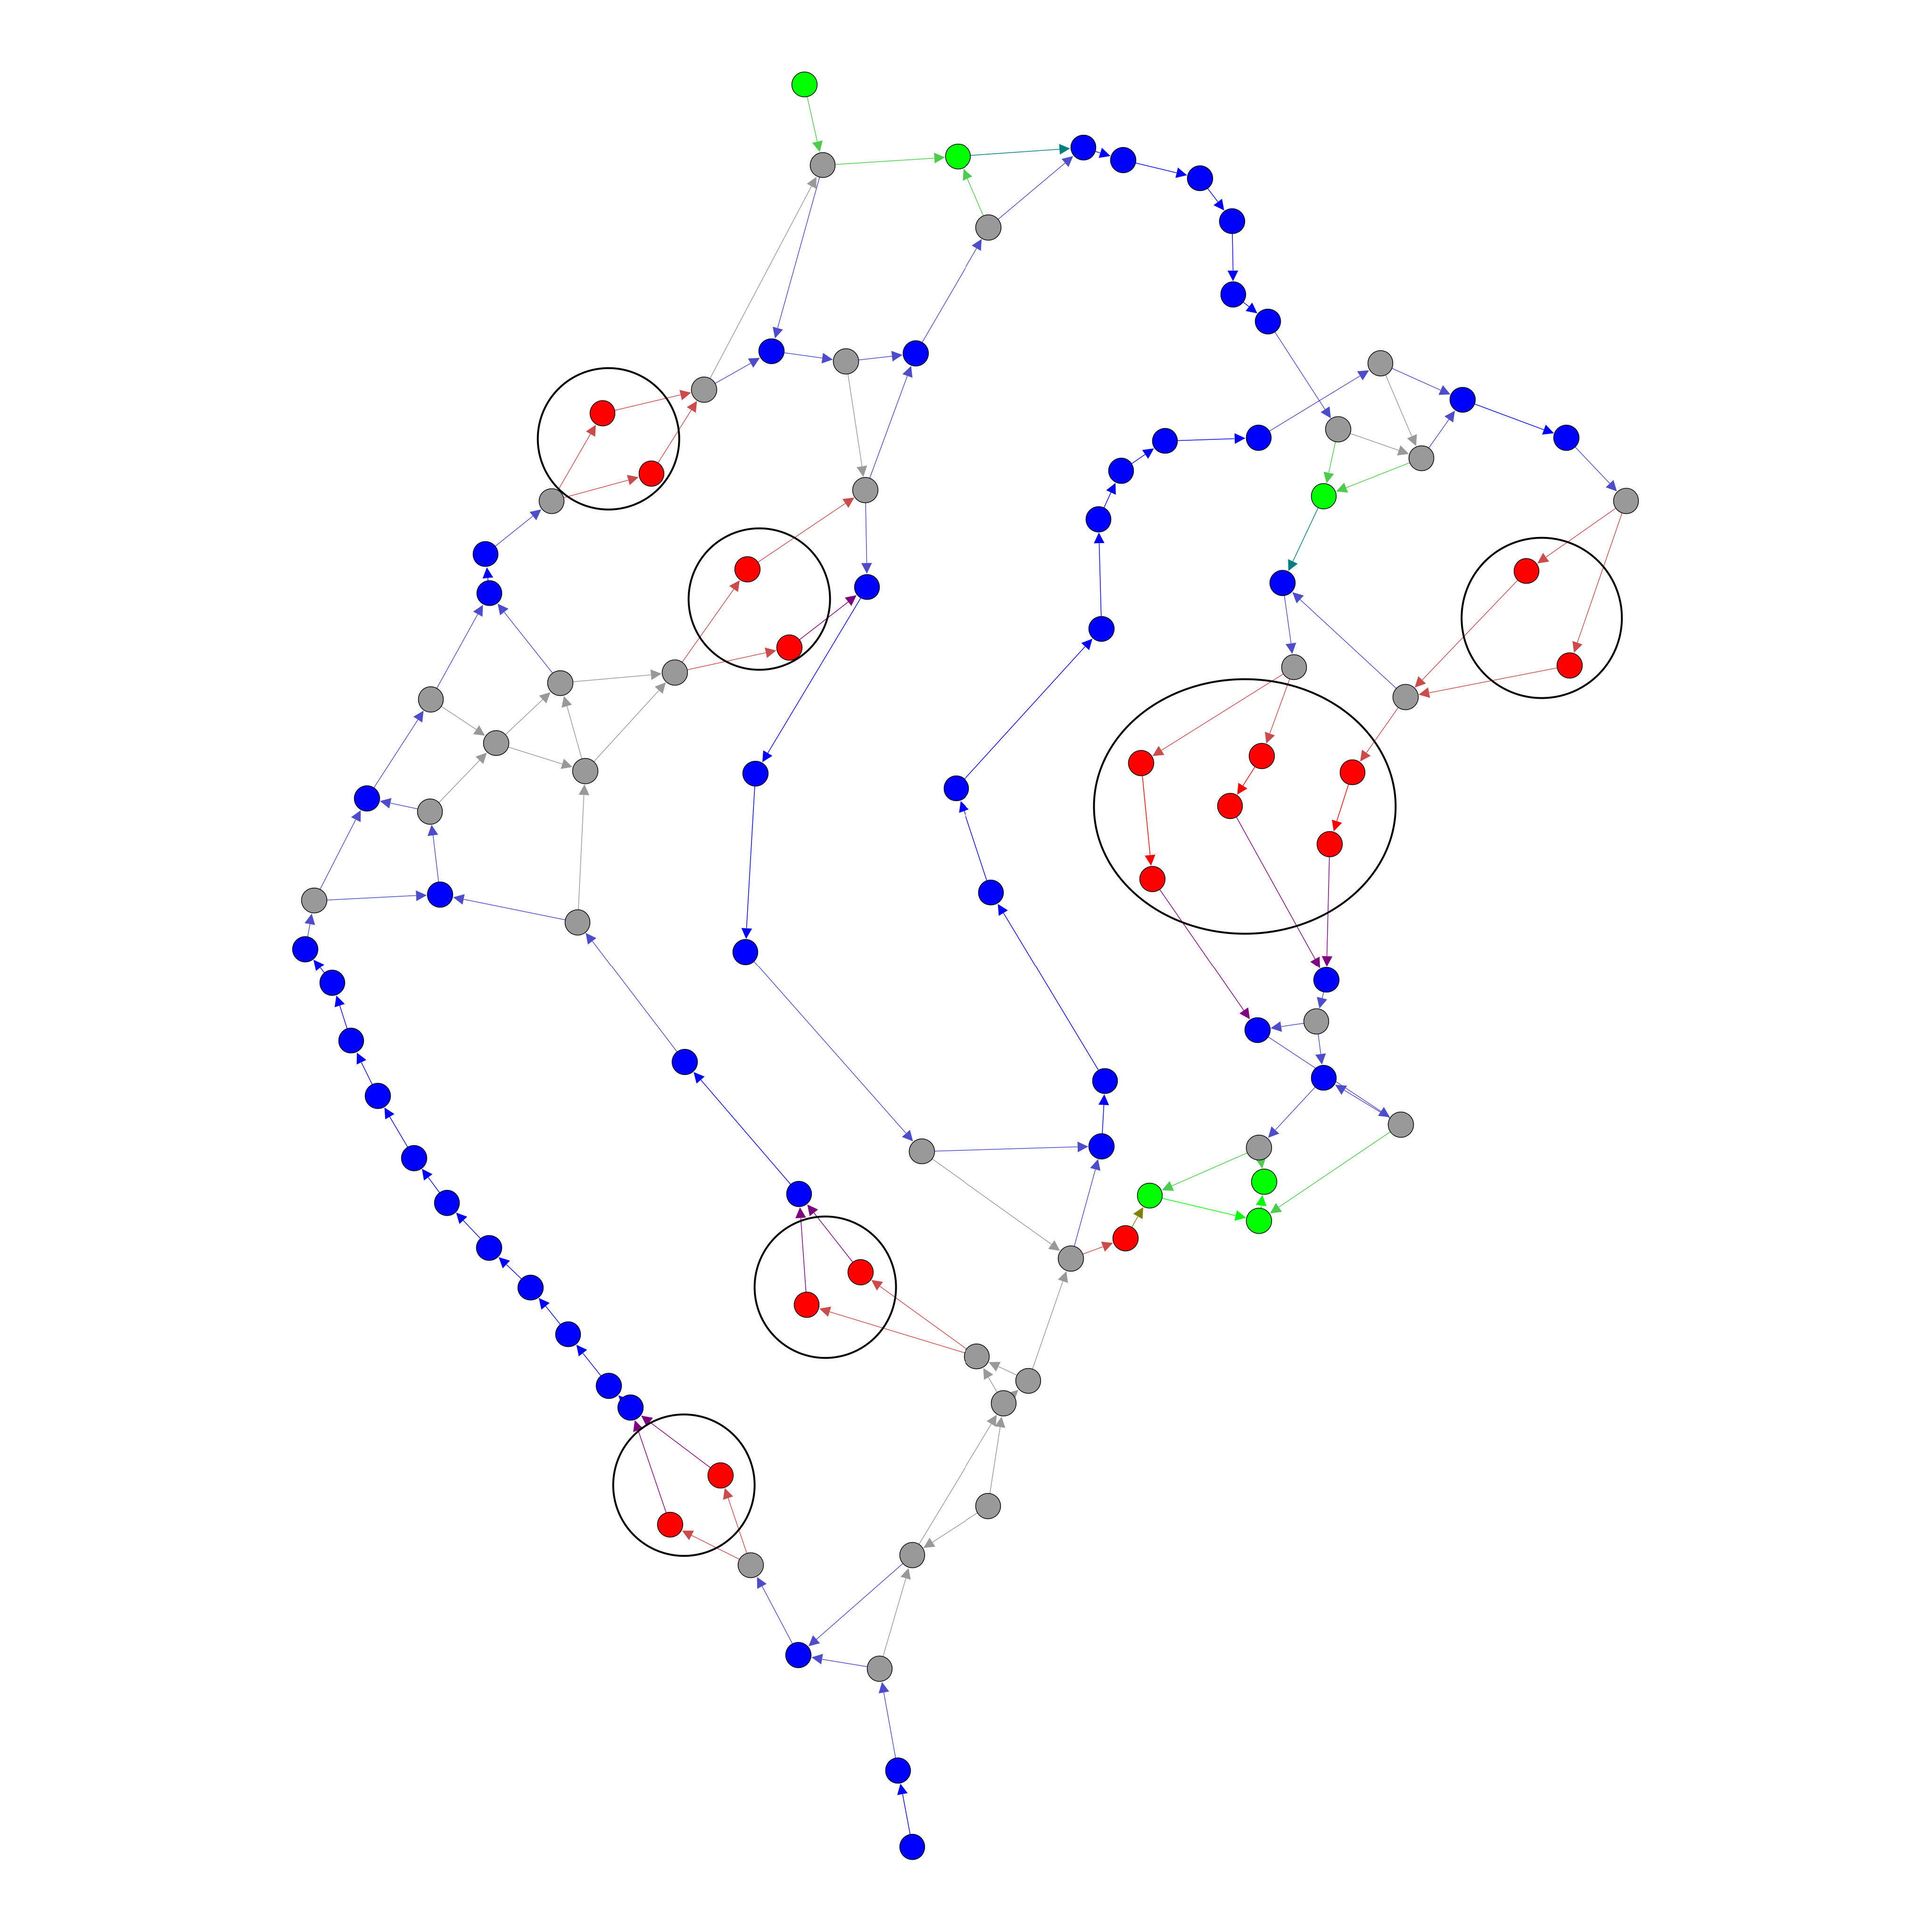
\includegraphics[scale=0.0375]{experimentation/deadlock/deadlock.png}}
	\caption{Potential deadlocks in MultiChain.}
	\label{fig:deadlock-double}
\end{figure}